\section{Computing with Reals}
\subsection{Overview}
\begin{frame}
  Different approaches to compute with real numbers on a computer
  \begin{itemize}[<+->]
      \item Floating-Point Arithmetic
      \item Arbitrary-Precision Arithmetic
      \item Interval Arithmetic
      \item Symbolic Computation
      \item \textbf{Exact Real Arithmetic}
  \end{itemize}
\end{frame}
\subsection{DAGs}
\begin{frame}[<+->][t,fragile]
    \frametitle{Computations via DAGs: Top-Down Approach}
  \begin{lstlisting}
    x = sqrt(x0)+(x1*x2);
  \end{lstlisting}
  \vspace{20pt}
  \begin{center}
        \begin{tikzpicture}[remember picture, overlay
            ,->,shorten >=1pt,auto,node distance=2.5cm,minimum
              size=0.8cm,main node/.style={circle,fill=yellow!20,draw,font=\sffamily\small}]
    
    \node<2->[main node] (1) {$+$};
    \node<2->[main node] (2) [below left of=1] {$\sqrt{}$};
    \node<2->[main node] (6) [below left of=2] {$x_0$};
    \node<2->[main node] (3) [below right of=1] {$\times$};
    \node<2->[main node] (4) [below left of=3] {$x_1$};
    \node<2->[main node] (5) [below right of=3] {$x_2$};

    \node<3->[color=red] at (0.0,0.7) {$2^{-n}$};
    \node<4->[color=red] at (-2.0,-1.1) {$2^{-(n+1)}$};
    \node<4->[color=red] at (2.0,-1.1) {$2^{-(n+1)}$};
    \node<5->[color=red] at (-4.0,-2.6) {$2^{-(n+2)}$};
    \node<5->[color=red] at (-0.0,-2.8) {$2^{-(n+3)}$};
    \node<5->[color=red] at (4.0,-2.8) {$2^{-(n+3)}$};
    \path<2->[every node/.style={font=\sffamily\small}]
    (1) edge (2)
    (2) edge (6)
    (1) edge (3)
    (3) edge (4)
    (3) edge (5);
  \end{tikzpicture}
\end{center}
\end{frame}
\begin{frame}[<+->][fragile]
  \frametitle{Computations via DAGs: Top-Down Approach}
  \begin{textblock*}{\paperwidth}(-20pt,60pt)
        \raggedright
      \begin{lstlisting}
        y = x[0];
        for(int i=1; i<=1000; i++)
          y += x[i];
        \end{lstlisting}
        \hspace{.5em}
  \end{textblock*}
  \vfill
  \begin{center}
    \onslide<2->{
      \begin{tikzpicture}[remember picture, overlay,
          ->,shorten >=1pt,auto,node distance=2.5cm,minimum
            size=0.8cm,main node/.style={circle,fill=yellow!20,draw,font=\sffamily\small}]
    \node[main node] (1) {$+$};
    \node[main node] (2) [below left of=1] {$x_0$};
    \node[main node] (3) [below right of=1] {$x_1$};
    \node[main node] (4) [above right of=1] {$+$};
    \node[minimum size=0.5cm] (8) at (0.9, 0.9) {$\cdots$};
    \node[main node,font=\sffamily\tiny] (5) [below right of=4] {$x_{999}$};
    \node[main node] (6) [above right of=4] {$+$};
    \node[main node] (7) [below right of=6] {$x_{N}$};
    \node<3->[color=red] at (3.5,4.2) {$2^{-n}$};
    \node<4->[color=red] at (1.7,2.4) {$2^{-(n+1)}$};
    \node<4->[color=red] at (5.4,2.4) {$2^{-(n+1)}$};
    \node<4->[color=red] at (3.5,0.8) {$2^{-(n+2)}$};
    \node<4->[color=red] at (0.0,0.8) {$2^{-(n+999)}$};
    \node<5->[color=red] at (1.5,-1.2) {$2^{-(n+1000)}$};
    \node<5->[color=red] at (-2.0,-1.2) {$2^{-(n+1000)}$};
    \path[every node/.style={font=\sffamily\small}]
    (1) edge (2)
    (1) edge (3)
    (4) edge (5)
    (6) edge (4)
    (4) edge (8)
    (8) edge (1)
    (6) edge (7);
  \end{tikzpicture}
  }
  \end{center}
\end{frame}
\begin{frame}
  \frametitle{Computations via DAGs: Bottom-Up Approach}
    \vfill
    \begin{center}
      \begin{tikzpicture}[remember picture, overlay,
            ->,shorten >=1pt,auto,node distance=2.5cm,minimum
              size=0.8cm,main node/.style={circle,fill=yellow!20,draw,font=\sffamily\small}]
      \node[main node] (1) {$+$};
      \node[main node] (2) [below left of=1] {$x_0$};
      \node[main node] (3) [below right of=1] {$x_1$};
      \node[main node] (4) [above right of=1] {$+$};
      \node[minimum size=0.5cm] (8) at (0.9, 0.9) {$\cdots$};
      \node[main node,font=\sffamily\tiny] (5) [below right of=4] {$x_{999}$};
      \node[main node] (6) [above right of=4] {$+$};
      \node[main node] (7) [below right of=6] {$x_{N}$};
      \node<5>[color=red] at (3.5,4.2) {$1000 \times 2^{-10}$};
      \node<6>[color=red] at (3.5,4.2) {$> 2^{-5}$};
      \node<4-6>[color=red] at (1.7,2.4) {$999 \times 2^{-10}$};
      \node<2-6>[color=red] at (5.4,2.4) {$2^{-10}$};
      \node<2-6>[color=red] at (3.5,0.8) {$2^{-10}$};
      \node<3-6>[color=red] at (0.0,0.8) {$2^{-9}$};
      \node<2-6>[color=red] at (1.5,-1.2) {$2^{-10}$};
      \node<2-6>[color=red] at (-2.0,-1.2) {$2^{-10}$};
      \node<10>[color=red] at (3.5,4.2) {$1000 \times 2^{-20}$};
      \node<11>[color=green] at (3.5,4.2) {$< 2^{-5}$};
      \node<9->[color=red] at (1.7,2.4) {$999 \times 2^{-20}$};
      \node<7->[color=red] at (5.4,2.4) {$2^{-20}$};
      \node<7->[color=red] at (3.5,0.8) {$2^{-20}$};
      \node<8->[color=red] at (0.0,0.8) {$2^{-19}$};
      \node<7->[color=red] at (1.5,-1.2) {$2^{-20}$};
      \node<7->[color=red] at (-2.0,-1.2) {$2^{-20}$};
      \path[every node/.style={font=\sffamily\small}]
      (1) edge (2)
      (1) edge (3)
      (4) edge (5)
      (6) edge (4)
      (4) edge (8)
      (8) edge (1)
      (6) edge (7);
    \end{tikzpicture}
  \end{center}
\end{frame}
\subsection{The iRRAM framework}
\begin{frame}
  \frametitle{The \irram Framework}
  \begin{itemize}[<+->]
    \item \irram is a \cc framework for exact real arithmetic written by Norbert M\"{u}ller from the University of Trier.
      \item The idea is similar to the bottom up approach.
    \item Building and saving the DAGs costs lots of memory for large computations.
    \item \irram does not build the DAGs.
    \item If at some point during the computation the precision is not sufficient, \irram recomputes the whole program from the start.
  \end{itemize}
\end{frame}
\begin{frame}
  \frametitle{Multivalued Functions}
  \large
  A multivalued function $f$ is allowed to have multiple valid outputs $f(x)$ for an argument $x$.
  \pause
  \vfill
  In practice, that means that the output may also depend on the internal representation of $x$
  and not only on the real number $x$.
  \pause
  \vfill
  The output of a multi-valued function can change from one iteration to another.
  To prevent a change of program flow, it is necessary to save the output of a multi-valued function (multi-valued cache).
\end{frame}
\begin{frame}
  \frametitle{Limits}
  \begin{itemize}[<+->]
    \item everything seen so far can also be done by symbolic computation.
    \item there is no need for computable analysis yet
    \item \irram also allows the user to define new real numbers and functions
  \end{itemize}
\end{frame}
\begin{frame}[<+->][fragile]
  \frametitle{Simple Limits}
  \begin{lstlisting}
  REAL limit (REAL f(int));
  \end{lstlisting}
  Defines a new \real from an algorithm to generate that real.
  \vfill
  \pause
  \begin{lstlisting}
  REAL limit (REAL a(int, const REAL&),
                      const REAL& x);
  \end{lstlisting}
  returns the value $f(x) = \lim_{n \to \infty} a(n,x)$.
  $a$ has to converge rapidly.
\end{frame}
